% python3 code_to_tex.py nyc25.py nyc25_tex && xelatex </dev/null spork_nyc25.tex
\documentclass[12pt]{article}

\usepackage[a5paper, landscape, margin=10mm]{geometry}
\usepackage{enumitem}
\usepackage{amsmath}
\usepackage{amssymb}
\usepackage{amsfonts}
\usepackage{placeins}
\usepackage{graphicx}
\usepackage{listings}
\usepackage{caption}
\usepackage{colortbl}
\usepackage[parfill]{parskip}
\usepackage[mathscr]{euscript}
\usepackage[usenames,dvipsnames,svgnames,table,hyperref]{xcolor}
\usepackage[hidelinks]{hyperref}
\usepackage{fontspec}
\usepackage{mdframed}

\setsansfont{FreeSans}
\setmonofont{Ubuntu Mono}
\renewcommand{\familydefault}{\sfdefault}

\hyphenation{WebGL}

\definecolor{webColor}{RGB}{0, 108, 174}
\newcommand{\web}[1]{{\color{webColor} \small \url{#1}}}
\newcommand{\webText}[2]{{\color{webColor} \href{#2}{#1}}}
\newcommand{\email}[2]{{\small \color{webColor} \textsf{\href{mailto:#1@#2}{#1[at]#2}}}}
\definecolor{titleColor}{RGB}{179, 0, 149}
\newcommand{\myTitle}[1]{{\large \color{titleColor} \hspace{-4mm} \textbf{\textsf{#1}}}}
\definecolor{subColor}{RGB}{179, 0, 149}
\newcommand{\mySub}[1]{\textsf{\color{subColor}#1}}
\definecolor{keyColor}{RGB}{170, 149, 0}
\newcommand{\myKey}[1]{\textbf{\color{keyColor}#1}}

\definecolor{redBoxFg}{RGB}{255, 0, 0}
\definecolor{redBoxBg}{RGB}{255, 218, 232}
\newcommand{\redBox}[1]{{\color{redBoxFg}\colorbox{redBoxBg}{#1}}}
\definecolor{yellowBoxFg}{RGB}{0, 0, 0}
\definecolor{yellowBoxBg}{RGB}{255, 232, 0}
\newcommand{\yellowBox}[1]{{\color{yellowBoxFg}\colorbox{yellowBoxBg}{#1}}}
\definecolor{greenBoxFg}{RGB}{0, 0, 0}
\definecolor{greenBoxBg}{RGB}{134, 210, 153}
\newcommand{\greenBox}[1]{{\color{greenBoxFg}\colorbox{greenBoxBg}{#1}}}
\definecolor{blueBoxFg}{RGB}{0, 0, 255}
\definecolor{blueBoxBg}{RGB}{218, 232, 255}
\newcommand{\blueBox}[1]{{\color{blueBoxFg}\colorbox{blueBoxBg}{#1}}}
\definecolor{violetBoxFg}{RGB}{0, 0, 0}
\definecolor{violetBoxBg}{RGB}{218, 204, 255}
\newcommand{\violetBox}[1]{{\color{violetBoxFg}\colorbox{violetBoxBg}{#1}}}

\mdfdefinestyle{MyFrame}{%
    linecolor=black,
    outerlinewidth=0pt,
    linewidth=0pt,
    innertopmargin=2.7pt,
    innerbottommargin=0pt,
    innerrightmargin=0pt,
    innerleftmargin=0pt,
        leftmargin = 0pt,
        rightmargin = 0pt}

\definecolor{lightttColor}{RGB}{69, 69, 80}
\newcommand{\lighttt}[1]{{\color{lightttColor}\texttt{#1}}}

\renewcommand*\labelenumi{(\theenumi)}
\renewcommand*{\theenumii}{\roman{enumii}}
\renewcommand*\labelenumii{\theenumii.}

\newcommand{\fixminipage}{\raggedright \setlength{\parskip}{0.3\baselineskip}}
\newcommand{\codeminipage}{\raggedright \setlength{\parskip}{0\baselineskip}}
\sloppy
\pagenumbering{gobble}


\begin{document}

\tikzstyle{smallnode} = [rectangle, minimum width=1.25cm, minimum height=1cm, text centered, text width=1.25cm, draw=black, fill=white]
\tikzstyle{smallishnode} = [rectangle, minimum width=2cm, minimum height=1cm, text centered, text width=2cm, draw=black, fill=white]
\tikzstyle{normalnode} = [rectangle, minimum width=3cm, minimum height=1cm, text centered, text width=3cm, draw=black, fill=white]
\tikzstyle{widenode} = [rectangle, minimum width=62mm, minimum height=8mm, text centered, text width=62mm, draw=black, fill=white]
\tikzstyle{bignode} = [rectangle, minimum width=3.5cm, minimum height=2cm, text centered, text width=3cm, draw=black, fill=white]
\tikzstyle{smemnode} = [rectangle, minimum width=3cm, minimum height=1cm, text centered, text width=3cm, draw=keyColorB, fill=white]
\tikzstyle{gmemnode} = [rectangle, minimum width=3cm, minimum height=1cm, text centered, text width=3cm, draw=keyColorA, fill=white]
\tikzstyle{smallishsmemnode} = [rectangle, minimum width=2cm, minimum height=1cm, text centered, text width=2cm, draw=keyColorB, fill=white]
\tikzstyle{arrow} = [thick,->,>=stealth]
\tikzstyle{line} = [thick]

\tikzstyle{rednode} = [normalnode, draw=redBoxFg, fill=redBoxBg, text=redBoxFg]
\tikzstyle{yellownode} = [normalnode, draw=yellowBoxFg, fill=yellowBoxBg, text=yellowBoxFg]
\tikzstyle{greennode} = [normalnode, draw=greenBoxFg, fill=greenBoxBg, text=greenBoxFg]
\tikzstyle{bluenode} = [normalnode, draw=blueBoxFg, fill=blueBoxBg, text=blueBoxFg]
\tikzstyle{violetnode} = [normalnode, draw=violetBoxFg, fill=violetBoxBg, text=violetBoxFg]

\tikzstyle{redstyle} = [draw=redBoxFg, fill=redBoxBg, text=redBoxFg]
\tikzstyle{yellowstyle} = [draw=yellowBoxFg, fill=yellowBoxBg, text=yellowBoxFg]
\tikzstyle{greenstyle} = [draw=greenBoxFg, fill=greenBoxBg, text=greenBoxFg]
\tikzstyle{bluestyle} = [draw=blueBoxFg, fill=blueBoxBg, text=blueBoxFg]
\tikzstyle{violetstyle} = [draw=violetBoxFg, fill=violetBoxBg, text=violetBoxFg]

\tikzstyle{Mnode} = [greennode, text width=55mm, minimum width=55mm, minimum height=7mm]
\tikzstyle{Nnode} = [violetnode, text width=7mm, minimum width=7mm, minimum height=7mm]

\tikzstyle{producer} = [yellownode, text width=64mm, minimum width=64mm, minimum height=14mm]
\tikzstyle{consumer} = [greennode, text width=20mm, minimum width=20mm, minimum height=14mm]
\tikzstyle{smallproducer} = [yellownode, text width=20mm, minimum width=20mm, minimum height=14mm]
\tikzstyle{copylatency} = [violetnode, text width=84mm, minimum width=84mm, minimum height=8mm]
\tikzstyle{ring} = [violetnode, text width=16mm, minimum width=1mm, minimum height=14mm]
\newcommand{\consumerBox}[1]{{\color{greenBoxFg}\colorbox{greenBoxBg}{#1}}}
\newcommand{\producerBox}[1]{{\color{yellowBoxFg}\colorbox{yellowBoxBg}{#1}}}

\myBiggerTitle{Exo-GPU}

\textbf{\hfill \large Safe, Imperative, User-schedulable Programming for Tensor Cores}

{\LARGE

\vfill

David Zhao Akeley

Yuka Ikarashi

Jonathan Ragan-Kelley

\hfill \myBiggerTitle{2025 MIT/Jane Street Symposium}}

%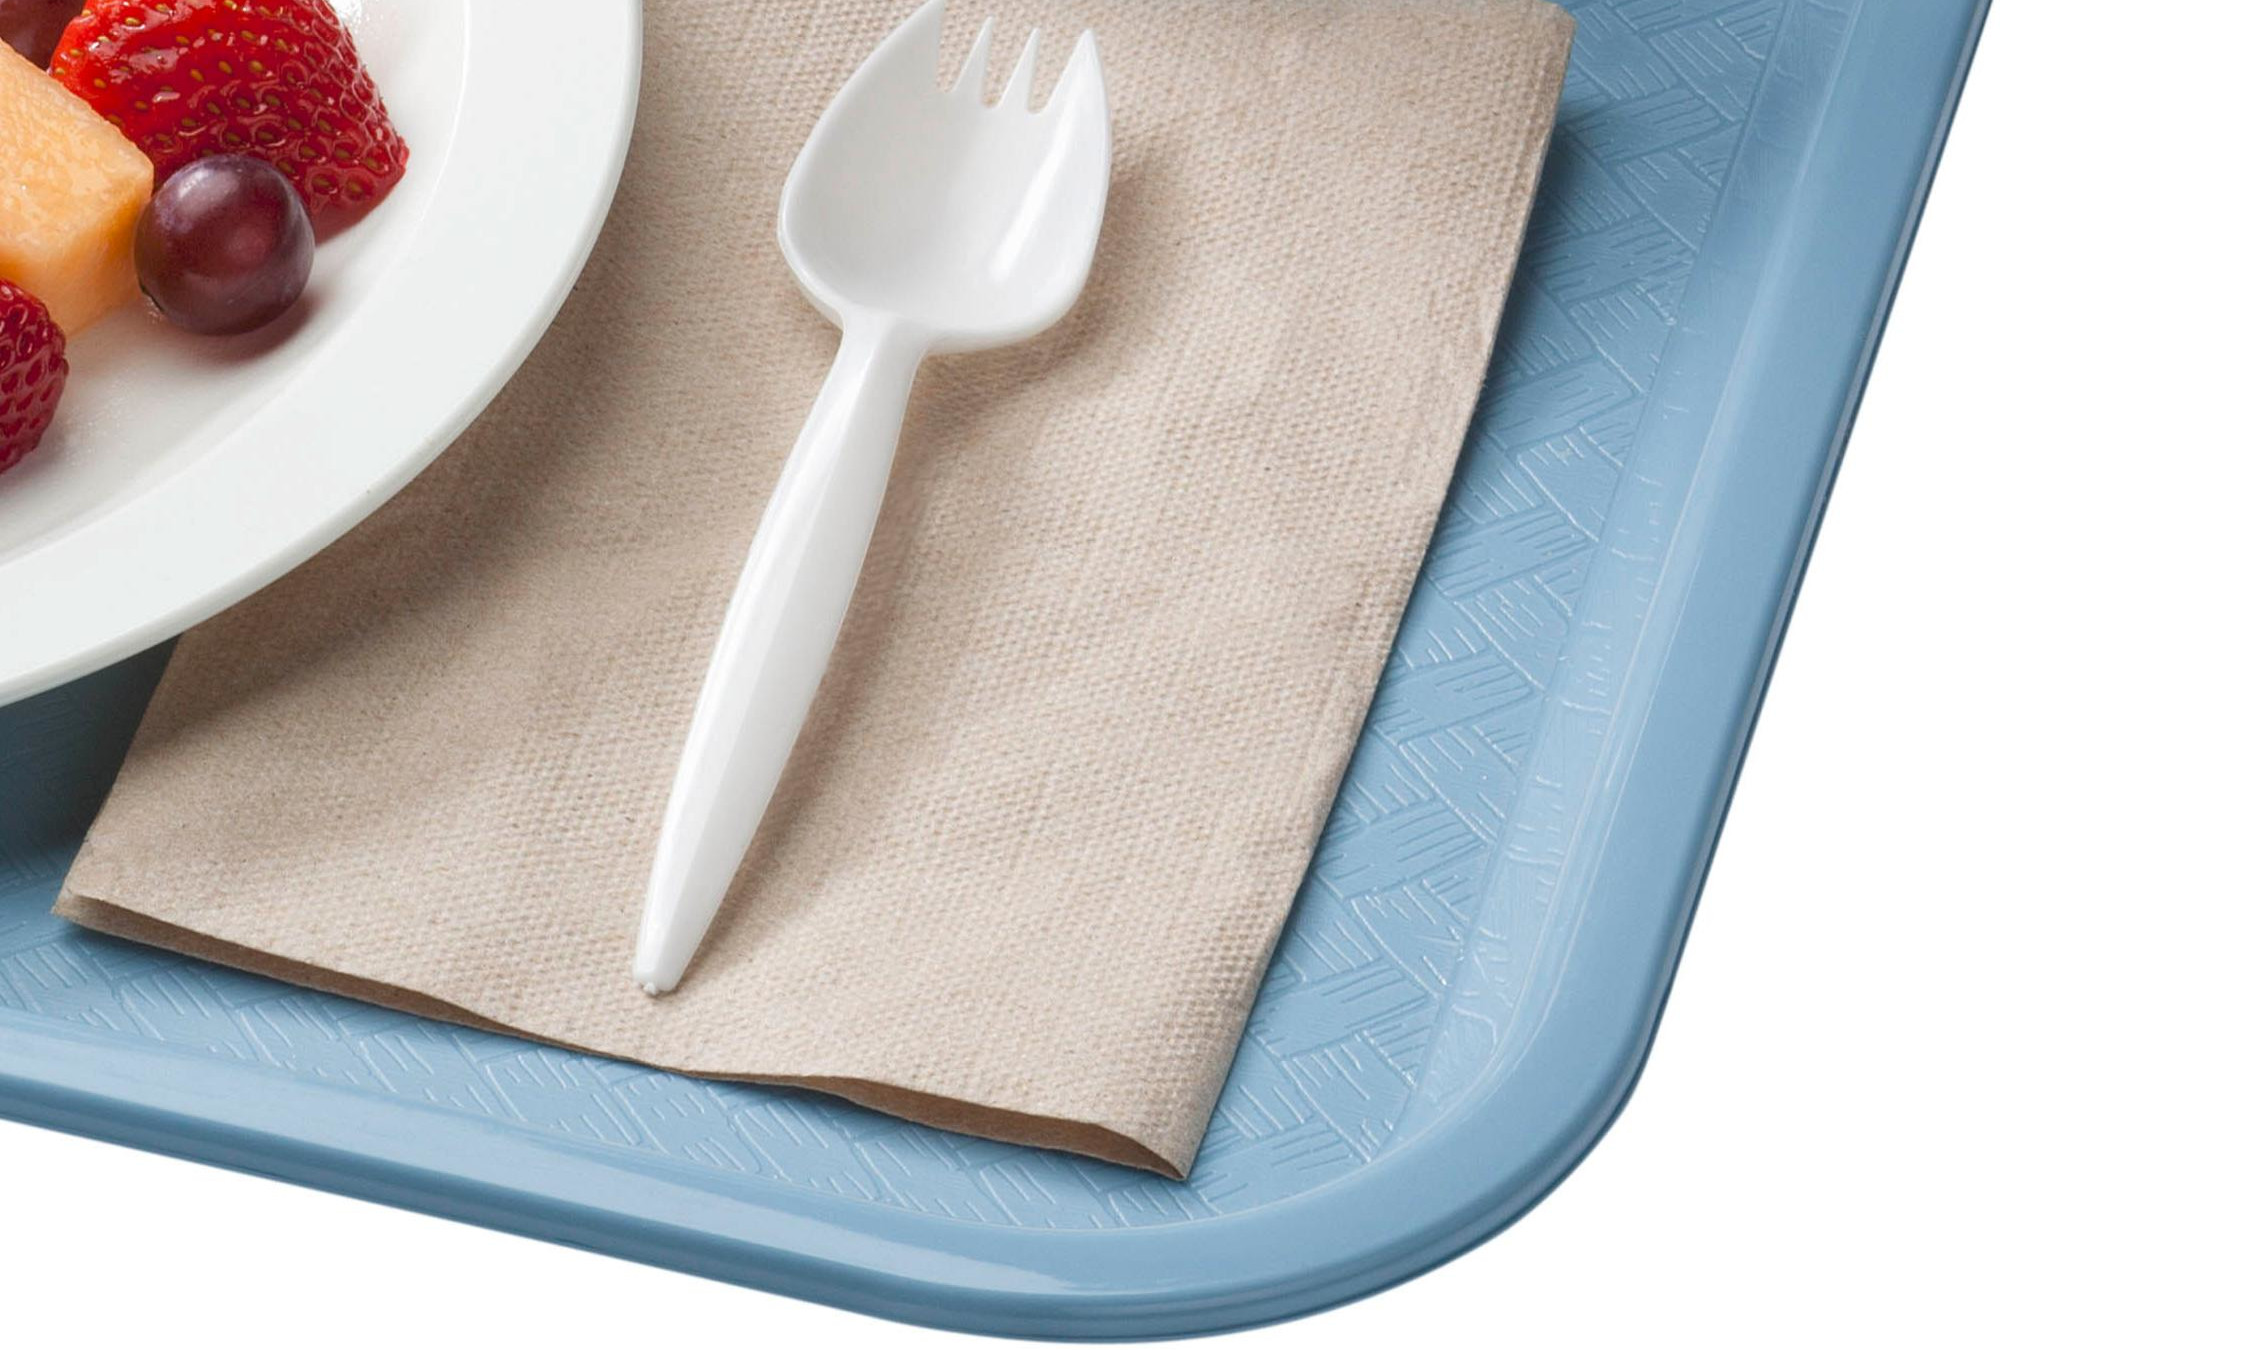
\includegraphics[width=\linewidth]{usda_spork.jpg}

\newpage
\myBiggerTitle{Challenge: SIMT Parallelism}

{\LARGE

Talk about launching blocks of threads

Talk about mapping work to threads

Diagram: vector add eye candy? y[threadIdx] += x[threadIdx]

}

\newpage
\myBiggerTitle{Challenge: Memory / Compute Overlap}

{\LARGE

Talk about overlapping memory and compute workloads

Contrast with SIMT
\begin{itemize}
  \item SIMT = threads doing the same thing
  \item Now, threads are doing something different
\end{itemize}

Diagram:
\begin{itemize}
  \item BAD: chain of memory and compute tasks
  \item GOOD: scary looking DAG of memory/compute tasks
\end{itemize}

Non-trivial dependency graph

}

\newpage
\myBiggerTitle{Challenge: Efficient Synchronization}

{\LARGE

Try not to stall threads

Don't screw up

Nondeterministic \& subtle bugs possible

}


\newpage
\myBiggerTitle{Goals}

{\LARGE

Imperative programming: for performance engineering, what-you-see-is-what-you-get.

}


\newpage
\myBiggerTitle{Exo: User-schedulable Language}

{\LARGE
Python-embedded imperative language

Rewrite rules: Python functions transform procedures
\begin{itemize}
  \item checked for functional equivalence
\end{itemize}

Instruction substitution: replace code blocks with instructions of equivalent functionality.

Exo exists today; extending it to model GPUs in a disciplined way.

}

\newpage
\myBiggerTitle{GEMM: Starting Code}

{\large
\input{nyc25_tex/cpu.0.tex}
}

{\LARGE
\texttt{@proc} (procedure) decorator captures Python AST\\transpiled to C or CUDA C++.

}

\newpage
\myBiggerTitle{GEMM: Starting Code}

{\large
\input{nyc25_tex/cpu.1.tex}
}

{\LARGE
Static typing:\\
annotate proc parameters, allocated variables.

}

\newpage
\myBiggerTitle{GEMM: Starting Code}

{\large
\input{nyc25_tex/cpu.2.tex}
}

{\LARGE
Memory annotation:\\
\texttt{@}-sign associates memory type for parameters \& declarations
}

\newpage
\myBiggerTitle{GEMM: Starting Code}

{\large
\input{nyc25_tex/cpu.3.tex}
}

{\LARGE
Most constructs map 1:1 to C.

\texttt{seq}-loop $\mapsto$ \texttt{for (int \textit{var} = lo; \textit{var} < hi; ++\textit{var})}

``sequential'' loop here; contrast to par loops later.

}

\newpage
\myBiggerTitle{GEMM: Divide Loop (M)}

{\large
\input{nyc25_tex/m_divide_loop.0.tex}
}

{\LARGE
Apply \texttt{divide\_loop} twice to tile the \greenBox{m} loop by 3.

}

\newpage
\myBiggerTitle{GEMM: Divide Loop (M)}

{\large
\input{nyc25_tex/m_divide_loop.1.tex}
}

{\LARGE
Exo rewrites all uses of \greenBox{\texttt{m}} in the loop body.

\texttt{m} $\mapsto$ \texttt{m2 * M1 + m1 * M0 + m0}

}

\newpage
\myBiggerTitle{GEMM: Divide Loop (M)}

{\large
\input{nyc25_tex/m_divide_loop.2.tex}
}

{\LARGE
Assume perfect tiling to simplify this talk (no tail case)

}

\newpage
\myBiggerTitle{GEMM: Divide Loop (N)}

{\large
\input{nyc25_tex/n_divide_loop.0.tex}
}

{\LARGE
Apply the same 3-level tiling to the \violetBox{n} loop.

}

\newpage
\myBiggerTitle{GEMM: Reorder Loops \yellowBox{\small SO read off how the code works now ``so we loop over''}}

{\large
\input{nyc25_tex/reorder_loops.0.tex}
}

{\LARGE
Exo checked all rewrites for correctness.

}

\newpage
\myBiggerTitle{GPU: Blocks \& Threads}

{\LARGE

Goal: Map tiles to different levels of the GPU hierarchy

\begin{itemize}
\item Demarcate CPU / CUDA code division
\item Change sequential loops to parallel
\item Use GPU memory
\end{itemize}

}

\begin{tikzpicture}[node distance=2mm]

\node (grid) [greennode, text width=5cm, minimum width=5cm] {grid};
\node (cpu) [left=of grid, xshift=-2cm] {\textbf{CPU}};
\draw [arrow] (cpu) -- node[above] {\textbf{launch}} (grid);
\node (cuda) [above=of grid, yshift=+4mm] {\textbf{CUDA Constructs}};
\node (exo) [right=of cuda, xshift=25mm] {\textbf{Exo-GPU Constructs}};

\node (cta0) [greennode, text width=20mm, minimum width=20mm, below=of grid, xshift=-15mm, yshift=-1cm] {block};
\node (cta1) [greennode, text width=20mm, minimum width=20mm, below=of grid, xshift=+15mm, yshift=-1cm] {block};

\node (thread0) [greennode, text width=16mm, minimum width=16mm, below=of cta0, yshift=-1cm, xshift=-32mm] {thread};
\node (thread1) [greennode, text width=16mm, minimum width=16mm, right=of thread0] {thread};
\node (thread2) [greennode, text width=16mm, minimum width=16mm, right=of thread1, xshift=22mm] {thread};

\draw [arrow] (grid.south) to[out=270, in=90] (cta0.north);
\draw [arrow] (grid.south) to[out=270, in=90] (cta1.north);

\draw [arrow] (cta0.south) to[out=270, in=90] (thread0.north);
\draw [arrow] (cta0.south) to[out=270, in=90] (thread1.north);
\draw [arrow] (cta0.south) to[out=270, in=90] (thread2.north);
\draw [dotted] (thread1.east) -- node[above] {\blueBox{blockDim}} (thread2.west);

\node (CudaDeviceFunction) [align=left, right=of grid, text width=100mm] {\large\texttt{\codecomment{\# CPU launches grid}\\with CudaDeviceFunction(\blueBox{blockDim=\textit{arg}}):\\~~\codecomment{\# Body lowered to CUDA C++}}\\};
\node (cudaTasks) [align=left, right=of cta1, text width=100mm] {\large\texttt{~~\codecomment{\# Parallel-for loop}\\~~\codecomment{\# generates per-block tasks}\\~~for \textit{iter} in cuda\_tasks(\textit{lo}, \textit{hi}):}\\};
\node (cudaThreads) [align=left, right=of thread2, text width=110mm] {\large\texttt{~~~~\codecomment{\# Somewhat more complicated}\\~~~~\codecomment{\# Assigns threads to iterations}\\~~~~for \textit{iter} in cuda\_threads(\textit{lo}, \textit{hi}, unit=\textit{u}):}\\};
\end{tikzpicture}

\newpage
\myBiggerTitle{GEMM: GPU and Memory \yellowBox{\small emph GPU/CPU code division, memory, remove GPU features here}}

{\large
\input{nyc25_tex/simple_gpu.0.tex}
}

{\LARGE
Move loops to CUDA device; switch to CUDA memory types.

}

\newpage
\myBiggerTitle{GEMM: GPU task (block) loops}

{\large
\input{nyc25_tex/simple_gpu.1.tex}
}

{\LARGE
Assign large \texttt{M1} $\times$ \texttt{N1} tiles to CUDA blocks.

\textit{NOTE: parallelism is not checked at this step;}

\textit{rewrites treat parallel loops as sequential.}

}

% \yellowBox{1 or 2 details one at a time, we need to frame mapping levels to loops...}

% \redBox{Add zoom-in code, no changes}

\newpage
\myBiggerTitle{GEMM: GPU thread loops}

{\large
\input{nyc25_tex/simple_gpu.2.tex}
}

{\LARGE
Assign small \texttt{M0} $\times$ \texttt{N0} tiles to CUDA threads.

\textit{NOTE: parallelism is not checked at this step;}

\textit{rewrites treat parallel loops as sequential.}

}

\newpage
\myBiggerTitle{GEMM: GPU thread loops}

{\large
\input{nyc25_tex/simple_gpu.3.tex}
}

{\LARGE
``unit'' to be explained shortly.

}

\newpage
\myBiggerTitle{GEMM: GPU per-thread work}

{\large
\input{nyc25_tex/simple_gpu.4.tex}
}

{\LARGE
Inner most loops stay as sequential.

Each thread loops over \texttt{M0} $\times$ \texttt{N0} iteration space.

}

\newpage
\myBiggerTitle{GPU Thread Loops}

{\large
\input{nyc25_tex/cuda_threads.0.tex}
}

{\LARGE
\texttt{unit} argument: \myKeyA{collective unit}.

Describes ``shape'' of grouping of threads (\myKeyA{thread collective}) assigned to execute each iteration of the loop.

Static property of each scope in Exo-GPU.

}

\newpage
\myBiggerTitle{GPU Thread Loops}

{\large
\input{nyc25_tex/cuda_threads.0.tex}
}

{\LARGE
Unlike other parallel loops, \texttt{cuda\_threads} cannot spawn more threads.
It just subdivides existing thread collectives.
}

\begin{tikzpicture}[node distance=2mm]
\node (cta) [bluenode, minimum width=30mm, minimum height=40mm] {block: 256 threads};

\node (m2) [Mnode, right=of cta, xshift=16mm] {\texttt{m1 = 2}; threads [32, 47]};
\node (m1) [Mnode, above=of m2] {\texttt{m1 = 1}; threads [16, 31]};
\node (m0) [Mnode, above=of m1] {\texttt{m1 = 0}; threads [0, 15]};
\node (m15) [Mnode, below=of m2, yshift=-9mm] {\texttt{m1 = 15}; threads [240, 255]};
\draw [arrow] (cta) -- node[above] {\texttt{for \yellowBox{m1}}} (m2);
\draw [dotted] (m2) -- (m15);
\node (m0n0) [Nnode, right=of m0, xshift=16mm] {0};
\node (m0n1) [Nnode, right=of m0n0] {1};
\node (m0n2) [Nnode, right=of m0n1] {2};
\node (m0n15) [Nnode, right=of m0n2, xshift=8mm] {15};
\node (m1n0) [Nnode, below=of m0n0] {16};
\node (m1n1) [Nnode, below=of m0n1] {17};
\node (m1n2) [Nnode, below=of m0n2] {18};
\node (m1n15) [Nnode, below=of m0n15] {31};
\node (m2n0) [Nnode, below=of m1n0] {32};
\node (m2n1) [Nnode, below=of m1n1] {33};
\node (m2n2) [Nnode, below=of m1n2] {34};
\node (m2n15) [Nnode, below=of m1n15] {47};
\node (m15n0) [Nnode, right=of m15, xshift=16mm] {240};
\node (m15n1) [Nnode, right=of m15n0] {241};
\node (m15n2) [Nnode, right=of m15n1] {242};
\node (m15n15) [Nnode, right=of m15n2, xshift=8mm] {255};
\draw [arrow] (m0) -- node[above] {\texttt{for \redBox{n1}}} (m0n0);
\draw [arrow] (m1) -- node[above] {\texttt{for \redBox{n1}}} (m1n0);
\draw [arrow] (m2) -- node[above] {\texttt{for \redBox{n1}}} (m2n0);
\draw [arrow] (m15) -- node[below] {\texttt{for \redBox{n1}}} (m15n0);
\draw [dotted] (m2n0) -- node[] {\texttt{n1=0}} (m15n0);
\draw [dotted] (m2n1) -- node[] {\texttt{n1=1}} (m15n1);
\draw [dotted] (m2n2) -- node[] {\texttt{n1=2}} (m15n2);
\draw [dotted] (m2n15) --node[] {\texttt{n1=15}} (m15n15);
\draw [dotted] (m0n2) -- (m0n15);
\draw [dotted] (m1n2) -- (m1n15);
\draw [dotted] (m2n2) -- (m2n15);
\draw [dotted] (m15n2) -- (m15n15);

\end{tikzpicture}

\newpage
\myBiggerTitle{Summary: Thread Block Tiling}

\begin{tikzpicture}[node distance=0mm]
\node (C) [normalnode, minimum width=90mm, minimum height=90mm] {\Huge C};
\node (cta0) [draw=black, minimum width=20mm, minimum height=20mm, above=of C, xshift=-33mm, yshift=-22mm] {block 0};
\node (cta1) [draw=black, minimum width=20mm, minimum height=20mm, above=of C, xshift=-11mm, yshift=-22mm] {block 1};
\node (cta2) [draw=black, minimum width=20mm, minimum height=20mm, above=of C, xshift=+11mm, yshift=-22mm] {block 2};
\node (cta3) [draw=black, minimum width=20mm, minimum height=20mm, above=of C, xshift=+33mm, yshift=-22mm] {...};
\node (cta4) [draw=black, minimum width=20mm, minimum height=20mm, above=of C, xshift=-33mm, yshift=-44mm] {...};
\node (cta8) [minimum width=20mm, minimum height=20mm, above=of C, xshift=-33mm, yshift=-66mm] {...};
\node (cta12) [minimum width=20mm, minimum height=20mm, above=of C, xshift=-33mm, yshift=-88mm] {...};
\node (M1) [right=of cta4] {\LARGE\greenBox{\texttt{M1}}};
\node (N1) [below=of cta4] {\LARGE~\violetBox{\texttt{N1}}};
\node (M) [right=of C] {\LARGE\greenBox{\texttt{~M~}}};
\node (N) [below=of C] {\LARGE\violetBox{\texttt{~N~}}};

\node (code) [text width=90mm, left=of C, align=left] {\large \input{nyc25_tex/loops.0.tex}\\};
\end{tikzpicture}

%\newline

\begin{center}
\begin{tikzpicture}[node distance=0mm]
\node (C) [normalnode, minimum width=90mm, minimum height=90mm] {\Huge C};
\node (cta0) [draw=black, minimum width=20mm, minimum height=20mm, above=of C, xshift=-33mm, yshift=-22mm] {block 0};
\node (cta1) [draw=black, minimum width=20mm, minimum height=20mm, above=of C, xshift=-11mm, yshift=-22mm] {block 1};
\node (cta2) [draw=black, minimum width=20mm, minimum height=20mm, above=of C, xshift=+11mm, yshift=-22mm] {block 2};
\node (cta3) [draw=black, minimum width=20mm, minimum height=20mm, above=of C, xshift=+33mm, yshift=-22mm] {...};
\node (cta4) [draw=black, minimum width=20mm, minimum height=20mm, above=of C, xshift=-33mm, yshift=-44mm] {...};
\node (cta8) [minimum width=20mm, minimum height=20mm, above=of C, xshift=-33mm, yshift=-66mm] {...};
\node (cta12) [minimum width=20mm, minimum height=20mm, above=of C, xshift=-33mm, yshift=-88mm] {...};
\node (M1) [right=of cta4] {\LARGE\greenBox{\texttt{M1}}};
\node (N1) [below=of cta4] {\LARGE~\violetBox{\texttt{N1}}};
\node (M) [right=of C] {\LARGE\greenBox{\texttt{~M~}}};
\node (N) [below=of C] {\LARGE\violetBox{\texttt{~N~}}};

\node (A0) [greenstyle, left=of cta0, minimum width=60mm, minimum height=20mm, xshift=-6mm] {\Huge A[...]};
\node (A1) [greenstyle, left=of cta4, minimum width=60mm, minimum height=20mm, xshift=-6mm] {\Huge A[...]};
\node (A2) [greenstyle, left=of cta8, minimum width=60mm, minimum height=20mm, xshift=-6mm] {\Huge A[...]};
\node (A3) [greenstyle, left=of cta12, minimum width=60mm, minimum height=20mm, xshift=-6mm] {\Huge A[...]};
\node (B0) [violetstyle, above=of cta0, minimum width=20mm, minimum height=24mm, yshift=6mm] {\Huge B[...]};
\node (B1) [violetstyle, above=of cta1, minimum width=20mm, minimum height=24mm, yshift=6mm] {\Huge B[...]};
\node (B2) [violetstyle, above=of cta2, minimum width=20mm, minimum height=24mm, yshift=6mm] {\Huge B[...]};
\node (B3) [violetstyle, above=of cta3, minimum width=20mm, minimum height=24mm, yshift=6mm] {\Huge B[...]};
\node (text) [left=of B0] {\myBiggerTitle{Block Matrix Product~~}};
\end{tikzpicture}
\end{center}

\newpage
\myBiggerTitle{Summary: Thread Tiling Within Block}

\begin{tikzpicture}[node distance=0mm]
\node (C) [draw=black, minimum width=90mm, minimum height=90mm] {\LARGE C (block tile)};

% above=of is hacky, would be nice to have anchor=center and at(C) so yshift isn't weird.
\node (t0) [minimum width=20mm, minimum height=20mm, above=of C, xshift=-33mm, yshift=-22mm, draw=black, align=center] {thread\\0};
\node (t1) [minimum width=20mm, minimum height=20mm, above=of C, xshift=-11mm, yshift=-22mm, draw=black, align=center] {thread\\1};
\node (t2) [minimum width=20mm, minimum height=20mm, above=of C, xshift=+11mm, yshift=-22mm] {...};
\node (t15) [minimum width=20mm, minimum height=20mm, above=of C, xshift=+33mm, yshift=-22mm, draw=black, align=center] {thread\\15};
\node (t16) [minimum width=20mm, minimum height=20mm, above=of C, xshift=-33mm, yshift=-44mm, draw=black, align=center] {thread\\16};
\node (t31) [minimum width=20mm, minimum height=20mm, above=of C, xshift=+33mm, yshift=-44mm, draw=black, align=center] {thread\\31};
\node (t32) [minimum width=20mm, minimum height=20mm, above=of C, xshift=-33mm, yshift=-66mm] {...};
\node (t240) [minimum width=20mm, minimum height=20mm, above=of C, xshift=-33mm, yshift=-88mm, draw=black, align=center] {thread\\240};
\node (t241) [minimum width=20mm, minimum height=20mm, above=of C, xshift=-11mm, yshift=-88mm, draw=black, align=center] {thread\\241};
\node (t242) [minimum width=20mm, minimum height=20mm, above=of C, xshift=+11mm, yshift=-88mm] {...};
\node (t255) [minimum width=20mm, minimum height=20mm, above=of C, xshift=+33mm, yshift=-88mm, draw=black, align=center] {thread\\255};
\node (t63) [minimum width=20mm, minimum height=20mm, above=of C, xshift=+33mm, yshift=-66mm] {...};
\node (M1) [right=of C] {\LARGE\greenBox{\texttt{M1}}};
\node (N1) [below=of C] {\LARGE\violetBox{\texttt{N1}}};
\node (M1) [right=of t16] {\LARGE\greenBox{\texttt{M0}}};
\node (N1) [below=of t16] {\LARGE\violetBox{\texttt{N0}}};

\node (code) [text width=90mm, left=of C, align=left] {\large \input{nyc25_tex/loops.1.tex}\\};
\end{tikzpicture}

{\LARGE \textit{Pedagogical: not the most efficient pattern.}}

% \newpage
\begin{tikzpicture}[node distance=0mm]
\node (C) [draw=black, minimum width=90mm, minimum height=90mm] {\LARGE C (block tile)};

% above=of is hacky, would be nice to have anchor=center and at(C) so yshift isn't weird.
\node (t0) [minimum width=20mm, minimum height=20mm, above=of C, xshift=-33mm, yshift=-22mm, draw=black, align=center] {thread\\0};
\node (t1) [minimum width=20mm, minimum height=20mm, above=of C, xshift=-11mm, yshift=-22mm, draw=black, align=center] {thread\\1};
\node (t2) [minimum width=20mm, minimum height=20mm, above=of C, xshift=+11mm, yshift=-22mm] {...};
\node (t15) [minimum width=20mm, minimum height=20mm, above=of C, xshift=+33mm, yshift=-22mm, draw=black, align=center] {thread\\15};
\node (t16) [minimum width=20mm, minimum height=20mm, above=of C, xshift=-33mm, yshift=-44mm, draw=black, align=center] {thread\\16};
\node (t31) [minimum width=20mm, minimum height=20mm, above=of C, xshift=+33mm, yshift=-44mm, draw=black, align=center] {thread\\31};
\node (t32) [minimum width=20mm, minimum height=20mm, above=of C, xshift=-33mm, yshift=-66mm] {...};
\node (t240) [minimum width=20mm, minimum height=20mm, above=of C, xshift=-33mm, yshift=-88mm, draw=black, align=center] {thread\\240};
\node (t241) [minimum width=20mm, minimum height=20mm, above=of C, xshift=-11mm, yshift=-88mm, draw=black, align=center] {thread\\241};
\node (t242) [minimum width=20mm, minimum height=20mm, above=of C, xshift=+11mm, yshift=-88mm] {...};
\node (t255) [minimum width=20mm, minimum height=20mm, above=of C, xshift=+33mm, yshift=-88mm, draw=black, align=center] {thread\\255};
\node (t63) [minimum width=20mm, minimum height=20mm, above=of C, xshift=+33mm, yshift=-66mm] {...};
\node (M1) [right=of C] {\LARGE\greenBox{\texttt{M1}}};
\node (N1) [below=of C] {\LARGE\violetBox{\texttt{N1}}};
\node (M1) [right=of t16] {\LARGE\greenBox{\texttt{M0}}};
\node (N1) [below=of t16] {\LARGE\violetBox{\texttt{N0}}};

\node (A) [greenstyle, left=of t240, minimum width=60mm, minimum height=20mm, xshift=-6mm] {\Huge A[...]};
\node (B) [violetstyle, above=of t15, minimum width=20mm, minimum height=24mm, yshift=6mm] {\Huge B[...]};
\draw [arrow] (A) to[in=90, out=90] (t240);
\draw [arrow] (A) to[in=90, out=90] (t241);
\draw [arrow] (A) to[in=90, out=90] (t242);
\draw [arrow] (A) to[in=90, out=90] (t255);
\draw [arrow] (B) to[in=180, out=180] (t15);
\draw [arrow] (B) to[in=180, out=180] (t31);
\draw [arrow] (B) to[in=180, out=180] (t63);
\draw [arrow] (B) to[in=180, out=180] (t255);
\node (text) [left=of B, text width=150mm, align=left] {\myBiggerTitle{Waste: Duplicate Reads in Block}};
\end{tikzpicture}

\newpage
\myBiggerTitle{Shared Memory: SMEM}

{\LARGE

SMEM: Per-thread-block \myKeyA{scratchpad}

Tile \blueBox{\texttt{k}} loop by \blueBox{\texttt{K0}} (\texttt{k $\mapsto$ k1 * K0 + k0})

Thread block cooperates to store A, B tiles in SMEM.

}

\vfill

\begin{center}
\begin{tikzpicture}[node distance=2mm]
\node (c) [normalnode, minimum width=50mm, minimum height=50mm] { \Huge C };
\node (eq) [right=of c] {$=$};
\node (a) [normalnode, minimum width=50mm, minimum height=50mm, right=of eq] { \Huge A };
\node (b) [normalnode, minimum width=50mm, minimum height=50mm, right=of a] { \Huge B };
\node (c0) [rednode, minimum width=10mm, minimum height=10mm, text width=12mm, xshift=-10mm, yshift=10mm] {thread block};
\node (a0) [greennode, minimum width=5mm, minimum height=10mm, text width=0mm, right=of c0, xshift=38mm] {};
\node (a1) [greennode, minimum width=5mm, minimum height=10mm, text width=0mm, right=of a0] {};
\node (a2) [greennode, minimum width=5mm, minimum height=10mm, text width=0mm, right=of a1] {};
\node (a3) [greennode, minimum width=5mm, minimum height=10mm, text width=0mm, right=of a2] {};
\node (a4) [greennode, minimum width=5mm, minimum height=10mm, text width=0mm, right=of a3] {};
\node (a5) [greennode, minimum width=5mm, minimum height=10mm, text width=0mm, right=of a4] {};
\node (a6) [greennode, minimum width=5mm, minimum height=10mm, text width=0mm, right=of a5] {};
\node (b0) [violetnode, minimum width=10mm, minimum height=5mm, text width=10mm, right=of a6, xshift=9mm, yshift=11.5mm] {};
\node (b1) [violetnode, minimum width=10mm, minimum height=5mm, text width=10mm, below=of b0] {};
\node (b2) [violetnode, minimum width=10mm, minimum height=5mm, text width=10mm, below=of b1] {};
\node (b3) [violetnode, minimum width=10mm, minimum height=5mm, text width=10mm, below=of b2] {};
\node (b4) [violetnode, minimum width=10mm, minimum height=5mm, text width=10mm, below=of b3] {};
\node (b5) [violetnode, minimum width=10mm, minimum height=5mm, text width=10mm, below=of b4] {};
\node (b6) [violetnode, minimum width=10mm, minimum height=5mm, text width=10mm, below=of b5] {};
\node (Am) [left=of a0] {\greenBox{\texttt{M1}}};
\node (Ak0) [above=of a0, yshift=-4mm] {\blueBox{\texttt{K0}}};
\node (Ak1) [above=of a1, yshift=-4mm] {\blueBox{\texttt{K0}}};
\node (Ak2) [above=of a2, yshift=-4mm] {\blueBox{\texttt{K0}}};
\node (Ak3) [above=of a3, yshift=-4mm] {\blueBox{\texttt{K0}}};
\node (Ak4) [above=of a4, yshift=-4mm] {\blueBox{\texttt{K0}}};
\node (Ak5) [above=of a5, yshift=-4mm] {\blueBox{\texttt{K0}}};
\node (Ak6) [above=of a6, yshift=-4mm] {\blueBox{\texttt{K0}}};
\node (Bn) [above=of b0] {\violetBox{\texttt{N1}}};
\node (Bk0) [left=of b0, xshift=4mm] {\blueBox{\texttt{K0}}};
\node (Bk1) [left=of b1, xshift=4mm] {\blueBox{\texttt{K0}}};
\node (Bk2) [left=of b2, xshift=4mm] {\blueBox{\texttt{K0}}};
\node (Bk3) [left=of b3, xshift=4mm] {\blueBox{\texttt{K0}}};
\node (Bk4) [left=of b4, xshift=4mm] {\blueBox{\texttt{K0}}};
\node (Bk5) [left=of b5, xshift=4mm] {\blueBox{\texttt{K0}}};
\node (Bk6) [left=of b6, xshift=4mm] {\blueBox{\texttt{K0}}};
\node (k) [above=of a] {\Large\texttt{k $\mapsto$ k1 * K0 + k0}};

\end{tikzpicture}
\end{center}

\newpage
\begin{center}
\Large
\begin{tikzpicture}[node distance=0mm]
\node (A) [draw=black, minimum width=40mm, minimum height=30mm, align=center] {Load A tile\\to SMEM\\(\texttt{\greenBox{M1} $\times$ \blueBox{K0}})};
\node (B) [draw=black, minimum width=40mm, minimum height=30mm, align=center, right=of A, xshift=20mm] {Load B tile\\to SMEM\\(\texttt{\blueBox{K0} $\times$ \violetBox{N1}})};
\node (accum) [draw=black, minimum width=40mm, minimum height=30mm, align=center, right=of B, xshift=20mm] {Accumulate\\Tile\\(\texttt{\blueBox{k0}} loop)};

\node (zero) [above=of A, yshift=8mm] {Zero accumulators};
\node (C) [above=of accum, yshift=8mm] {Write out C};

\draw [arrow] (zero) -- (A);
\draw [arrow] (accum) -- (C);
\draw [arrow] (A) -- (B);
\draw [arrow] (B) -- (accum);
\draw [arrow] (accum) to[in=40, out=140] node[below] (k1) {\blueBox{\texttt{k1}} loop} (A);

\node (text) [below=of B] {\textbf{All steps are thread-block-cooperative.}};
\end{tikzpicture}
\end{center}

\vfill
\hrule
\vfill

\begin{center}
\begin{tikzpicture}[node distance=2mm]
\node (c) [normalnode, minimum width=50mm, minimum height=50mm] { \Huge C };
\node (eq) [right=of c] {$=$};
\node (a) [normalnode, minimum width=50mm, minimum height=50mm, right=of eq] { \Huge A };
\node (b) [normalnode, minimum width=50mm, minimum height=50mm, right=of a] { \Huge B };
\node (c0) [rednode, minimum width=10mm, minimum height=10mm, text width=12mm, xshift=-10mm, yshift=10mm] {thread block};
\node (a0) [greennode, minimum width=5mm, minimum height=10mm, text width=0mm, right=of c0, xshift=38mm] {};
\node (a1) [greennode, minimum width=5mm, minimum height=10mm, text width=0mm, right=of a0] {};
\node (a2) [greennode, minimum width=5mm, minimum height=10mm, text width=0mm, right=of a1] {};
\node (a3) [greennode, minimum width=5mm, minimum height=10mm, text width=0mm, right=of a2] {};
\node (a4) [greennode, minimum width=5mm, minimum height=10mm, text width=0mm, right=of a3] {};
\node (a5) [greennode, minimum width=5mm, minimum height=10mm, text width=0mm, right=of a4] {};
\node (a6) [greennode, minimum width=5mm, minimum height=10mm, text width=0mm, right=of a5] {};
\node (b0) [violetnode, minimum width=10mm, minimum height=5mm, text width=10mm, right=of a6, xshift=9mm, yshift=11.5mm] {};
\node (b1) [violetnode, minimum width=10mm, minimum height=5mm, text width=10mm, below=of b0] {};
\node (b2) [violetnode, minimum width=10mm, minimum height=5mm, text width=10mm, below=of b1] {};
\node (b3) [violetnode, minimum width=10mm, minimum height=5mm, text width=10mm, below=of b2] {};
\node (b4) [violetnode, minimum width=10mm, minimum height=5mm, text width=10mm, below=of b3] {};
\node (b5) [violetnode, minimum width=10mm, minimum height=5mm, text width=10mm, below=of b4] {};
\node (b6) [violetnode, minimum width=10mm, minimum height=5mm, text width=10mm, below=of b5] {};
\node (Am) [left=of a0] {\greenBox{\texttt{M1}}};
\node (Ak0) [above=of a0, yshift=-4mm] {\blueBox{\texttt{K0}}};
\node (Ak1) [above=of a1, yshift=-4mm] {\blueBox{\texttt{K0}}};
\node (Ak2) [above=of a2, yshift=-4mm] {\blueBox{\texttt{K0}}};
\node (Ak3) [above=of a3, yshift=-4mm] {\blueBox{\texttt{K0}}};
\node (Ak4) [above=of a4, yshift=-4mm] {\blueBox{\texttt{K0}}};
\node (Ak5) [above=of a5, yshift=-4mm] {\blueBox{\texttt{K0}}};
\node (Ak6) [above=of a6, yshift=-4mm] {\blueBox{\texttt{K0}}};
\node (Bn) [above=of b0] {\violetBox{\texttt{N1}}};
\node (Bk0) [left=of b0, xshift=4mm] {\blueBox{\texttt{K0}}};
\node (Bk1) [left=of b1, xshift=4mm] {\blueBox{\texttt{K0}}};
\node (Bk2) [left=of b2, xshift=4mm] {\blueBox{\texttt{K0}}};
\node (Bk3) [left=of b3, xshift=4mm] {\blueBox{\texttt{K0}}};
\node (Bk4) [left=of b4, xshift=4mm] {\blueBox{\texttt{K0}}};
\node (Bk5) [left=of b5, xshift=4mm] {\blueBox{\texttt{K0}}};
\node (Bk6) [left=of b6, xshift=4mm] {\blueBox{\texttt{K0}}};
\node (k) [above=of a] {\Large\texttt{k $\mapsto$ k1 * K0 + k0}};

\end{tikzpicture}
\end{center}

\newpage
\myBiggerTitle{GEMM: Restructuring}

{\large
\input{nyc25_tex/simple_gpu.5.tex}
}

{\LARGE
TODO: divide \texttt{k} loop \& reorder

TODO: factor out of \blueBox{\texttt{k1}} loop: \texttt{accum = 0}, write to \texttt{C}

}

\newpage
\myBiggerTitle{GEMM: Lift Alloc \& Expand Dim}

{\large
\input{nyc25_tex/simple_gpu.6.tex}
}

{\LARGE
Scope of \texttt{accum} variable is too small.

Need to lift it out to thread-block scope.

}

\newpage
\myBiggerTitle{GEMM: Lift Alloc \& Expand Dim}

{\large
\input{nyc25_tex/expand_dim.0.tex}
}

{\LARGE
Lift the allocation of \redBox{\texttt{accum}} into thread-block-scope\\
(just below \violetBox{\texttt{cuda\_tasks}} loops)
}

\newpage
\myBiggerTitle{GEMM: Lift Alloc \& Expand Dim}

{\large
\input{nyc25_tex/expand_dim.1.tex}
}

{\LARGE
Expand dim: each iteration uses its own index of \texttt{accum}
}

\newpage
\myBiggerTitle{GEMM: Loop Fission}

{\large
\input{nyc25_tex/expand_dim.2.tex}
}

{\LARGE
We will split the loop at the indicated locations, retaining the loop structure.
}

\newpage

{\large
\input{nyc25_tex/fission.0.tex}
}

\newpage
\myBiggerTitle{GEMM: K Loop Tiling}

{\large
\input{nyc25_tex/fission.1.tex}
}

{\LARGE
We'll focus on the accumulate loops for the rest of the talk.

}

\newpage
\myBiggerTitle{GEMM: K Loop Tiling}

{\large
\input{nyc25_tex/smem_broken.0.tex}
}

%% {\LARGE
%% Split k loop, and reorder sequential \blueBox{k1} loop outwards
%% }

\begin{center}
\Large
\begin{tikzpicture}[node distance=0mm]
\node (A) [draw=black, minimum width=40mm, minimum height=30mm, align=center] {Load A tile\\to SMEM\\(\texttt{\greenBox{M1} $\times$ \blueBox{K0}})};
\node (B) [draw=black, minimum width=40mm, minimum height=30mm, align=center, right=of A, xshift=20mm] {Load B tile\\to SMEM\\(\texttt{\blueBox{K0} $\times$ \violetBox{N1}})};
\node (accum) [draw=black, minimum width=40mm, minimum height=30mm, align=center, right=of B, xshift=20mm] {Accumulate\\Tile\\(\texttt{\blueBox{k0}} loop)};

\node (zero) [above=of A, yshift=8mm] {Zero accumulators};
\node (C) [above=of accum, yshift=8mm] {Write out C};

\draw [arrow] (zero) -- (A);
\draw [arrow] (accum) -- (C);
\draw [arrow] (A) -- (B);
\draw [arrow] (B) -- (accum);
\draw [arrow] (accum) to[in=40, out=140] node[below] (k1) {\blueBox{\texttt{k1}} loop} (A);

\end{tikzpicture}
\end{center}

\newpage
\myBiggerTitle{GEMM: Stage in SMEM}

{\large
\input{nyc25_tex/smem_broken.1.tex}
}

{\LARGE
Stage $\texttt{M1} \times \texttt{K0}$ tile of \greenBox{\texttt{A}}, $\texttt{K0} \times \texttt{N1}$ tile of \violetBox{\texttt{B}} in shared memory.

\texttt{A\_smem}, \texttt{B\_smem} replace \texttt{A} and \texttt{B} in the loop body.

}

\newpage
\myBiggerTitle{GEMM: Stage in SMEM}

{\large
\input{nyc25_tex/smem_broken.2.tex}
}

{\LARGE
The compiler generates loops to load the shared memory tile.

\texttt{seq} loops by default -- we will fix this!

}

\newpage
\myBiggerTitle{GEMM: Stage in SMEM}

{\large
\input{nyc25_tex/smem_in_order.0.tex}
}

{\LARGE
Divide \& Parallelize the load-shared-memory loops.
}

\newpage
\myBiggerTitle{GEMM: Stage in SMEM}

{\large
\input{nyc25_tex/smem_in_order.1.tex}
}

{\LARGE
Add synchronization:\\
All threads in the thread block wait for each other.
}

\newpage
\myBiggerTitle{``Classic'' GPU GEMM Summary}

{\LARGE
Synchronization required:\\
Thread that loaded a value to SMEM isn't the same as the one that uses it.

}

\vfill
\hrule
\vfill

\begin{center}
\Large
\begin{tikzpicture}[node distance=0mm]
\node (A) [greenstyle, minimum width=40mm, minimum height=30mm, align=center] {Load A tile\\to SMEM\\(\texttt{M1 $\times$ K0})};
\node (B) [violetstyle, minimum width=40mm, minimum height=30mm, align=center, right=of A, xshift=8mm] {Load B tile\\to SMEM\\(\texttt{K0 $\times$ N1})};
\node (raw) [yellowstyle, minimum width=10mm, minimum height=30mm, right=of B, xshift=8mm] {};
\node (accum) [draw=black, minimum width=40mm, minimum height=30mm, align=center, right=of raw, xshift=8mm] {Accumulate\\Tile\\(\texttt{\blueBox{k0}} loop)};
\node (war) [yellowstyle, minimum width=10mm, minimum height=30mm, right=of accum, xshift=8mm] {};

\node (zero) [above=of A, yshift=8mm] {Zero accumulators};
\node (C) [above=of war, yshift=8mm] {Write out C};

\draw [arrow] (zero) -- (A);
\draw [arrow] (war) -- (C);
\draw [arrow] (A) -- (B);
\draw [arrow] (B) -- (raw);
\draw [arrow] (raw) -- (accum);
\draw [arrow] (accum) -- (war);
\draw [arrow] ($(war.north)$) to[in=20, out=160] node[below]{\blueBox{\texttt{k1}} loop} ($(A.north)$);

\node (raw_caption) [below=of raw, align=center] {\textbf{Sync:}\\\textbf{RAW Hazard}};
\node (war_caption) [below=of war, align=center] {\textbf{Sync:}\\\textbf{WAR Hazard}};
\node (text) [below=of A, align=center, xshift=12mm] {\textbf{All steps are thread-}\\\textbf{block-cooperative.}};

\end{tikzpicture}
\end{center}

\newpage
\myBiggerTitle{``Classic'' GPU GEMM Summary}

{\LARGE
First sync: wait for SMEM tile to fill\\(RAW: read-after-write)

Second sync: don't overwrite until all SMEM reads are done\\(WAR: write-after-read)

}

\vfill
\hrule
\vfill

\begin{center}
\Large
\begin{tikzpicture}[node distance=0mm]
\node (A) [greenstyle, minimum width=40mm, minimum height=30mm, align=center] {Load A tile\\to SMEM\\(\texttt{M1 $\times$ K0})};
\node (B) [violetstyle, minimum width=40mm, minimum height=30mm, align=center, right=of A, xshift=8mm] {Load B tile\\to SMEM\\(\texttt{K0 $\times$ N1})};
\node (raw) [yellowstyle, minimum width=10mm, minimum height=30mm, right=of B, xshift=8mm] {};
\node (accum) [draw=black, minimum width=40mm, minimum height=30mm, align=center, right=of raw, xshift=8mm] {Accumulate\\Tile\\(\texttt{\blueBox{k0}} loop)};
\node (war) [yellowstyle, minimum width=10mm, minimum height=30mm, right=of accum, xshift=8mm] {};

\node (zero) [above=of A, yshift=8mm] {Zero accumulators};
\node (C) [above=of war, yshift=8mm] {Write out C};

\draw [arrow] (zero) -- (A);
\draw [arrow] (war) -- (C);
\draw [arrow] (A) -- (B);
\draw [arrow] (B) -- (raw);
\draw [arrow] (raw) -- (accum);
\draw [arrow] (accum) -- (war);
\draw [arrow] ($(war.north)$) to[in=20, out=160] node[below]{\blueBox{\texttt{k1}} loop} ($(A.north)$);

\node (raw_caption) [below=of raw, align=center] {\textbf{Sync:}\\\textbf{RAW Hazard}};
\node (war_caption) [below=of war, align=center] {\textbf{Sync:}\\\textbf{WAR Hazard}};
\node (text) [below=of A, align=center, xshift=12mm] {\textbf{All steps are thread-}\\\textbf{block-cooperative.}};

\end{tikzpicture}
\end{center}

\newpage
\myBiggerTitle{``Classic'' GPU GEMM Summary}

{\LARGE
Syncs strictly separate data movement workloads\\and compute workloads.

Not optimal.

}

\vfill
\hrule
\vfill

\begin{center}
\Large
\begin{tikzpicture}[node distance=0mm]
\node (A) [greenstyle, minimum width=40mm, minimum height=30mm, align=center] {Load A tile\\to SMEM\\(\texttt{M1 $\times$ K0})};
\node (B) [violetstyle, minimum width=40mm, minimum height=30mm, align=center, right=of A, xshift=8mm] {Load B tile\\to SMEM\\(\texttt{K0 $\times$ N1})};
\node (raw) [yellowstyle, minimum width=10mm, minimum height=30mm, right=of B, xshift=8mm] {};
\node (accum) [draw=black, minimum width=40mm, minimum height=30mm, align=center, right=of raw, xshift=8mm] {Accumulate\\Tile\\(\texttt{\blueBox{k0}} loop)};
\node (war) [yellowstyle, minimum width=10mm, minimum height=30mm, right=of accum, xshift=8mm] {};

\node (zero) [above=of A, yshift=8mm] {Zero accumulators};
\node (C) [above=of war, yshift=8mm] {Write out C};

\draw [arrow] (zero) -- (A);
\draw [arrow] (war) -- (C);
\draw [arrow] (A) -- (B);
\draw [arrow] (B) -- (raw);
\draw [arrow] (raw) -- (accum);
\draw [arrow] (accum) -- (war);
\draw [arrow] ($(war.north)$) to[in=20, out=160] node[below]{\blueBox{\texttt{k1}} loop} ($(A.north)$);

\node (raw_caption) [below=of raw, align=center] {\textbf{Sync:}\\\textbf{RAW Hazard}};
\node (war_caption) [below=of war, align=center] {\textbf{Sync:}\\\textbf{WAR Hazard}};
\node (text) [below=of A, align=center, xshift=12mm] {\textbf{All steps are thread-}\\\textbf{block-cooperative.}};

% \node (text) [below=of B] {All steps are thread-block-cooperative.};
\end{tikzpicture}
\end{center}


\newpage
\myBiggerTitle{Async Copies}

{\LARGE
Ampere (sm\_80) introduced async copy instructions\\
(GMEM $\to$ SMEM)

Execution continues on without waiting for the copy to finish.

}

{\Large
\input{nyc25_tex/cp_async_pseudocode.0.tex}
}

{\LARGE
\myKeyA{Overlapping:} issue non-dependent \myKeyA{compute} work while copies are in-flight.
}

\newpage
\myBiggerTitle{Timelines}

{\LARGE
Most synchronization instructions \myKeyA{don't wait} for cp.async.

\myKeyA{Timelines:} categorize instrs by \myKeyA{synchronization needed}.

\begin{itemize}
  \item \textbf{\texttt{cuda\_in\_order}}: most CUDA instructions
  \item \textbf{\texttt{Sm80\_cp\_async}}: \texttt{cp.async} (special syncs needed)
  \item Others for H100 (not in this talk)
\end{itemize}

}

\newpage
\myBiggerTitle{Exo-GPU Synchronization}

{\LARGE
Parameterize Exo-GPU synchronization with timelines:

\begin{center}
  \texttt{Fence(\myKeyA{L1}, \myKeyB{L2})}
\end{center}

\textbf{Semi-declarative}; user specifies intended effect:

\begin{center}
prior \myKeyA{L1}-timeline instrs $\xrightarrow{\textbf{SYNC}}$ future \myKeyB{L2}-timeline instrs
\end{center}

Compiler chooses exact instructions.

Otherwise imperative\\(executes in program order with surrounding instructions)

}

\newpage
\myBiggerTitle{GEMM: Prepare for cp.async}

{\large
\input{nyc25_tex/smem_in_order.2.tex}
}

{\LARGE
Current main loop:
only \textbf{\texttt{cuda\_in\_order}} instructions used,
so \textbf{\texttt{Fence}} is parameterized with \texttt{cuda\_in\_order}.
}

\newpage
\myBiggerTitle{GEMM: Prepare for cp.async}

{\large
\input{nyc25_tex/smem_in_order.3.tex}
}

{\LARGE
TODO: replace these GMEM$\to$SMEM copies with cp.async.
}

\newpage
\myBiggerTitle{GEMM: Prepare for cp.async}

{\large
\input{nyc25_tex/smem_in_order.4.tex}
}

{\LARGE
TODO: update timeline parameters for synchronization.
}

\newpage
\myBiggerTitle{GEMM: cp.async (Substitute Instruction)}

{\large
\input{nyc25_tex/cp_async.0.tex}
}

{\LARGE

Replace \texttt{A\_smem[\codecomment{...}] = A[\codecomment{...}]} and \texttt{B\_smem[\codecomment{...}] = B[\codecomment{...}]}\\with cp.async instructions.

Exo allows the rewrite, because the substituted functionality, \textit{ignoring concurrency}, is equivalent.

}

\newpage
\myBiggerTitle{GEMM: cp.async (CudaAsync block)}

{\large
\input{nyc25_tex/cp_async.1.tex}
}

{\LARGE

Such instructions must be wrapped in a CudaAsync block.

}

\newpage
\myBiggerTitle{GEMM: cp.async (Synchronization)}

{\large
\input{nyc25_tex/cp_async.2.tex}
}

{\LARGE

Update the timeline parameters for synchronization.

}

\newpage
\myBiggerTitle{More to do: Overlap Compute/Memory}
\begin{center}
\Large
\begin{tikzpicture}[node distance=0mm]
\node (A) [greenstyle, minimum width=40mm, minimum height=30mm, align=center] {Load A tile\\to SMEM\\(\texttt{M1 $\times$ K0})};
\node (B) [violetstyle, minimum width=40mm, minimum height=30mm, align=center, right=of A, xshift=8mm] {Load B tile\\to SMEM\\(\texttt{K0 $\times$ N1})};
\node (raw) [yellowstyle, minimum width=10mm, minimum height=30mm, right=of B, xshift=8mm] {};
\node (accum) [draw=black, minimum width=40mm, minimum height=30mm, align=center, right=of raw, xshift=8mm] {Accumulate\\Tile\\(\texttt{\blueBox{k0}} loop)};
\node (war) [yellowstyle, minimum width=10mm, minimum height=30mm, right=of accum, xshift=8mm] {};

\node (zero) [above=of A, yshift=8mm] {Zero accumulators};
\node (C) [above=of war, yshift=8mm] {Write out C};

\draw [arrow] (zero) -- (A);
\draw [arrow] (war) -- (C);
\draw [arrow] (A) -- (B);
\draw [arrow] (B) -- (raw);
\draw [arrow] (raw) -- (accum);
\draw [arrow] (accum) -- (war);
\draw [arrow] ($(war.north)$) to[in=20, out=160] node[below]{\blueBox{\texttt{k1}} loop} ($(A.north)$);

\node (raw_caption) [below=of raw, align=center] {\textbf{Sync:}\\\textbf{RAW Hazard}};
\node (war_caption) [below=of war, align=center] {\textbf{Sync:}\\\textbf{WAR Hazard}};
\node (text) [below=of A, align=center, xshift=12mm] {\textbf{All steps are thread-}\\\textbf{block-cooperative.}};

\end{tikzpicture}
\end{center}


\newpage
\myBiggerTitle{More to do: Overlap Compute/Memory}
\begin{center}
\Large
\begin{tikzpicture}[node distance=0mm]
\node (A) [greenstyle, minimum width=40mm, minimum height=30mm, align=center] {Load A tile\\to SMEM\\(\texttt{M1 $\times$ K0})};
\node (B) [violetstyle, minimum width=40mm, minimum height=30mm, align=center, right=of A, xshift=8mm] {Load B tile\\to SMEM\\(\texttt{K0 $\times$ N1})};
\node (raw) [yellowstyle, minimum width=10mm, minimum height=30mm, right=of B, xshift=8mm] {};
\node (accum) [draw=black, minimum width=40mm, minimum height=30mm, align=center, right=of raw, xshift=8mm] {Accumulate\\Tile\\(\texttt{\blueBox{k0}} loop)};
\node (war) [yellowstyle, minimum width=10mm, minimum height=30mm, right=of accum, xshift=8mm] {};

\node (zero) [above=of A, yshift=8mm] {Zero accumulators};
\node (C) [above=of war, yshift=8mm] {Write out C};

\draw [arrow] (zero) -- (A);
\draw [arrow] (war) -- (C);
\draw [arrow] (A) -- (B);
\draw [arrow] (B) -- (raw);
\draw [arrow] (raw) -- (accum);
\draw [arrow] (accum) -- (war);
\draw [arrow] ($(war.north)$) to[in=20, out=160] node[below]{\blueBox{\texttt{k1}} loop} ($(A.north)$);

\node (raw_caption) [below=of raw, align=center] {\textbf{Sync:}\\\textbf{RAW Hazard}};
\node (war_caption) [below=of war, align=center] {\textbf{Sync:}\\\textbf{WAR Hazard}};
\node (text) [below=of A, align=center, xshift=12mm] {\textbf{All steps are thread-}\\\textbf{block-cooperative.}};

\node (async) [redstyle, right=of A, xshift=-20mm, yshift=-12mm, align=center, text width=40mm, minimum height=25mm] {\textbf{NOW WITH cp.async!}};
\end{tikzpicture}
\end{center}
\hrule
{\LARGE
We need to \myKeyA{delay} the accumulate step to a future iteration to make room for overlapping work!

}

\newpage
\myBiggerTitle{Producer/Consumer Dependencies}

{
\Large
\begin{tikzpicture}[node distance=0mm]
\node (A0) [greenstyle, minimum width=28mm, minimum height=12mm, xshift=11mm] {Load A};
\node (B0) [violetstyle, minimum width=28mm, minimum height=12mm, below=of A0] {Load B};

\node (A1) [greenstyle, minimum width=28mm, minimum height=12mm, xshift=11mm, right=of A0] {Load A};
\node (B1) [violetstyle, minimum width=28mm, minimum height=12mm, below=of A1] {Load B};

\node (A2) [greenstyle, minimum width=28mm, minimum height=12mm, xshift=11mm, right=of A1] {Load A};
\node (B2) [violetstyle, minimum width=28mm, minimum height=12mm, below=of A2] {Load B};

\node (A3) [greenstyle, minimum width=28mm, minimum height=12mm, xshift=11mm, right=of A2] {Load A};
\node (B3) [violetstyle, minimum width=28mm, minimum height=12mm, below=of A3] {Load B};

\node (A4) [greenstyle, minimum width=28mm, minimum height=12mm, xshift=11mm, right=of A3] {Load A};
\node (B4) [violetstyle, minimum width=28mm, minimum height=12mm, below=of A4] {Load B};

\node (A5) [greenstyle, minimum width=28mm, minimum height=12mm, xshift=11mm, right=of A4] {Load A};
\node (B5) [violetstyle, minimum width=28mm, minimum height=12mm, below=of A5] {Load B};

\node (A6) [greenstyle, minimum width=28mm, minimum height=12mm, xshift=11mm, right=of A5] {Load A};
\node (B6) [violetstyle, minimum width=28mm, minimum height=12mm, below=of A6] {Load B};

\node (A7) [greenstyle, minimum width=28mm, minimum height=12mm, xshift=11mm, right=of A6] {Load A};
\node (B7) [violetstyle, minimum width=28mm, minimum height=12mm, below=of A7] {Load B};

\node (C0) [minimum width=28mm, minimum height=21mm, below=of B0, yshift=-11mm] {};
\node (C1) [draw=black, minimum width=28mm, minimum height=21mm, below=of B1, yshift=-11mm] {compute};
\node (C2) [draw=black, minimum width=28mm, minimum height=21mm, below=of B2, yshift=-11mm] {compute};
\node (C3) [draw=black, minimum width=28mm, minimum height=21mm, below=of B3, yshift=-11mm] {compute};
\node (C4) [draw=black, minimum width=28mm, minimum height=21mm, below=of B4, yshift=-11mm] {compute};
\node (C5) [draw=black, minimum width=28mm, minimum height=21mm, below=of B5, yshift=-11mm] {compute};
\node (C6) [draw=black, minimum width=28mm, minimum height=21mm, below=of B6, yshift=-11mm] {compute};

\draw [arrow] ($(A0.south east)$) to[out=0, in=180] (C1);
\draw [arrow] ($(A1.south east)$) to[out=0, in=180] (C2);
\draw [arrow] ($(A2.south east)$) to[out=0, in=180] (C3);
\draw [arrow] ($(A3.south east)$) to[out=0, in=180] (C4);
\draw [arrow] ($(A4.south east)$) to[out=0, in=180] (C5);
\draw [arrow] ($(A5.south east)$) to[out=0, in=180] (C6);


\end{tikzpicture}
}

\hrule

{\LARGE
Loop skew: delay \myKeyA{consumption} (compute) of SMEM data by one \blueBox{\texttt{k1}} iteration from SMEM load.

}

\newpage
\myBiggerTitle{Producer/Consumer Dependencies}

{
\Large
\begin{tikzpicture}[node distance=0mm]
\node (A0) [greenstyle, minimum width=28mm, minimum height=12mm, xshift=11mm] {Load A};
\node (B0) [violetstyle, minimum width=28mm, minimum height=12mm, below=of A0] {Load B};

\node (A1) [greenstyle, minimum width=28mm, minimum height=12mm, xshift=11mm, right=of A0] {Load A};
\node (B1) [violetstyle, minimum width=28mm, minimum height=12mm, below=of A1] {Load B};

\node (A2) [greenstyle, minimum width=28mm, minimum height=12mm, xshift=11mm, right=of A1] {Load A};
\node (B2) [violetstyle, minimum width=28mm, minimum height=12mm, below=of A2] {Load B};

\node (A3) [greenstyle, minimum width=28mm, minimum height=12mm, xshift=11mm, right=of A2] {Load A};
\node (B3) [violetstyle, minimum width=28mm, minimum height=12mm, below=of A3] {Load B};

\node (A4) [greenstyle, minimum width=28mm, minimum height=12mm, xshift=11mm, right=of A3] {Load A};
\node (B4) [violetstyle, minimum width=28mm, minimum height=12mm, below=of A4] {Load B};

\node (A5) [greenstyle, minimum width=28mm, minimum height=12mm, xshift=11mm, right=of A4] {Load A};
\node (B5) [violetstyle, minimum width=28mm, minimum height=12mm, below=of A5] {Load B};

\node (A6) [greenstyle, minimum width=28mm, minimum height=12mm, xshift=11mm, right=of A5] {Load A};
\node (B6) [violetstyle, minimum width=28mm, minimum height=12mm, below=of A6] {Load B};

\node (A7) [greenstyle, minimum width=28mm, minimum height=12mm, xshift=11mm, right=of A6] {Load A};
\node (B7) [violetstyle, minimum width=28mm, minimum height=12mm, below=of A7] {Load B};

\node (C0) [minimum width=28mm, minimum height=21mm, below=of B0, yshift=-11mm] {};
\node (C1) [draw=black, minimum width=28mm, minimum height=21mm, below=of B1, yshift=-11mm] {compute};
\node (C2) [draw=black, minimum width=28mm, minimum height=21mm, below=of B2, yshift=-11mm] {compute};
\node (C3) [draw=black, minimum width=28mm, minimum height=21mm, below=of B3, yshift=-11mm] {compute};
\node (C4) [draw=black, minimum width=28mm, minimum height=21mm, below=of B4, yshift=-11mm] {compute};
\node (C5) [draw=black, minimum width=28mm, minimum height=21mm, below=of B5, yshift=-11mm] {compute};
\node (C6) [draw=black, minimum width=28mm, minimum height=21mm, below=of B6, yshift=-11mm] {compute};

\draw [arrow] ($(A0.south east)$) to[out=0, in=180] (C1);
\draw [arrow] ($(A1.south east)$) to[out=0, in=180] (C2);
\draw [arrow] ($(A2.south east)$) to[out=0, in=180] (C3);
\draw [arrow] ($(A3.south east)$) to[out=0, in=180] (C4);
\draw [arrow] ($(A4.south east)$) to[out=0, in=180] (C5);
\draw [arrow] ($(A5.south east)$) to[out=0, in=180] (C6);

\node (buf0) [below=of k0, xshift=8mm] {\textbf{Ring Buffer:}};
\node (buf1) [below=of k1, draw=black] {Slot 0};
\node (buf2) [below=of k2] {Slot 1};
\node (buf3) [below=of k3] {Slot 2};
\node (buf4) [below=of k4, draw=black] {Slot 0};
\node (buf5) [below=of k5] {Slot 1};



\end{tikzpicture}
}

\hrule

{\LARGE
Need to transform SMEM into a \myKeyA{ring buffer}.

One slot may be being filled while another is consumed.

}

\newpage
\myBiggerTitle{Producer/Consumer Dependencies}

{
\Large
\begin{tikzpicture}[node distance=0mm]
\node (A0) [greenstyle, minimum width=28mm, minimum height=12mm, xshift=11mm] {Load A};
\node (B0) [violetstyle, minimum width=28mm, minimum height=12mm, below=of A0] {Load B};

\node (A1) [greenstyle, minimum width=28mm, minimum height=12mm, xshift=11mm, right=of A0] {Load A};
\node (B1) [violetstyle, minimum width=28mm, minimum height=12mm, below=of A1] {Load B};

\node (A2) [greenstyle, minimum width=28mm, minimum height=12mm, xshift=11mm, right=of A1] {Load A};
\node (B2) [violetstyle, minimum width=28mm, minimum height=12mm, below=of A2] {Load B};

\node (A3) [greenstyle, minimum width=28mm, minimum height=12mm, xshift=11mm, right=of A2] {Load A};
\node (B3) [violetstyle, minimum width=28mm, minimum height=12mm, below=of A3] {Load B};

\node (A4) [greenstyle, minimum width=28mm, minimum height=12mm, xshift=11mm, right=of A3] {Load A};
\node (B4) [violetstyle, minimum width=28mm, minimum height=12mm, below=of A4] {Load B};

\node (A5) [greenstyle, minimum width=28mm, minimum height=12mm, xshift=11mm, right=of A4] {Load A};
\node (B5) [violetstyle, minimum width=28mm, minimum height=12mm, below=of A5] {Load B};

\node (A6) [greenstyle, minimum width=28mm, minimum height=12mm, xshift=11mm, right=of A5] {Load A};
\node (B6) [violetstyle, minimum width=28mm, minimum height=12mm, below=of A6] {Load B};

\node (A7) [greenstyle, minimum width=28mm, minimum height=12mm, xshift=11mm, right=of A6] {Load A};
\node (B7) [violetstyle, minimum width=28mm, minimum height=12mm, below=of A7] {Load B};

\node (C0) [minimum width=28mm, minimum height=21mm, below=of B0, yshift=-11mm] {};
\node (C1) [draw=black, minimum width=28mm, minimum height=21mm, below=of B1, yshift=-11mm] {compute};
\node (C2) [draw=black, minimum width=28mm, minimum height=21mm, below=of B2, yshift=-11mm] {compute};
\node (C3) [draw=black, minimum width=28mm, minimum height=21mm, below=of B3, yshift=-11mm] {compute};
\node (C4) [draw=black, minimum width=28mm, minimum height=21mm, below=of B4, yshift=-11mm] {compute};
\node (C5) [draw=black, minimum width=28mm, minimum height=21mm, below=of B5, yshift=-11mm] {compute};
\node (C6) [draw=black, minimum width=28mm, minimum height=21mm, below=of B6, yshift=-11mm] {compute};

\draw [arrow] ($(A0.south east)$) to[out=0, in=180] (C1);
\draw [arrow] ($(A1.south east)$) to[out=0, in=180] (C2);
\draw [arrow] ($(A2.south east)$) to[out=0, in=180] (C3);
\draw [arrow] ($(A3.south east)$) to[out=0, in=180] (C4);
\draw [arrow] ($(A4.south east)$) to[out=0, in=180] (C5);
\draw [arrow] ($(A5.south east)$) to[out=0, in=180] (C6);

\node (buf0) [below=of k0, xshift=8mm] {\textbf{Ring Buffer:}};
\node (buf1) [below=of k1, draw=black] {Slot 0};
\node (buf2) [below=of k2] {Slot 1};
\node (buf3) [below=of k3] {Slot 2};
\node (buf4) [below=of k4, draw=black] {Slot 0};
\node (buf5) [below=of k5] {Slot 1};


\draw [arrow] ($(C1.east) + (0, 6mm)$) to[out=40, in=220] ($(B3.west)$);
\draw [arrow] ($(C2.east) + (0, 6mm)$) to[out=40, in=220] ($(B4.west)$);
\draw [arrow] ($(C3.east) + (0, 6mm)$) to[out=40, in=220] ($(B5.west)$);
\draw [arrow] ($(C4.east) + (0, 6mm)$) to[out=40, in=220] ($(B6.west)$);


\end{tikzpicture}
}

\hrule

{\LARGE
WAR hazard: require syncs before re-using ring buffer slots.

}


\newpage
\myBiggerTitle{Producer/Consumer Dependencies}

{
\Large
\begin{tikzpicture}[node distance=0mm]
\node (A0) [greenstyle, minimum width=28mm, minimum height=12mm, xshift=11mm] {Load A};
\node (B0) [violetstyle, minimum width=28mm, minimum height=12mm, below=of A0] {Load B};

\node (A1) [greenstyle, minimum width=28mm, minimum height=12mm, xshift=11mm, right=of A0] {Load A};
\node (B1) [violetstyle, minimum width=28mm, minimum height=12mm, below=of A1] {Load B};

\node (A2) [greenstyle, minimum width=28mm, minimum height=12mm, xshift=11mm, right=of A1] {Load A};
\node (B2) [violetstyle, minimum width=28mm, minimum height=12mm, below=of A2] {Load B};

\node (A3) [greenstyle, minimum width=28mm, minimum height=12mm, xshift=11mm, right=of A2] {Load A};
\node (B3) [violetstyle, minimum width=28mm, minimum height=12mm, below=of A3] {Load B};

\node (A4) [greenstyle, minimum width=28mm, minimum height=12mm, xshift=11mm, right=of A3] {Load A};
\node (B4) [violetstyle, minimum width=28mm, minimum height=12mm, below=of A4] {Load B};

\node (A5) [greenstyle, minimum width=28mm, minimum height=12mm, xshift=11mm, right=of A4] {Load A};
\node (B5) [violetstyle, minimum width=28mm, minimum height=12mm, below=of A5] {Load B};

\node (A6) [greenstyle, minimum width=28mm, minimum height=12mm, xshift=11mm, right=of A5] {Load A};
\node (B6) [violetstyle, minimum width=28mm, minimum height=12mm, below=of A6] {Load B};

\node (A7) [greenstyle, minimum width=28mm, minimum height=12mm, xshift=11mm, right=of A6] {Load A};
\node (B7) [violetstyle, minimum width=28mm, minimum height=12mm, below=of A7] {Load B};

\node (C0) [minimum width=28mm, minimum height=21mm, below=of B0, yshift=-11mm] {};
\node (C1) [draw=black, minimum width=28mm, minimum height=21mm, below=of B1, yshift=-11mm] {compute};
\node (C2) [draw=black, minimum width=28mm, minimum height=21mm, below=of B2, yshift=-11mm] {compute};
\node (C3) [draw=black, minimum width=28mm, minimum height=21mm, below=of B3, yshift=-11mm] {compute};
\node (C4) [draw=black, minimum width=28mm, minimum height=21mm, below=of B4, yshift=-11mm] {compute};
\node (C5) [draw=black, minimum width=28mm, minimum height=21mm, below=of B5, yshift=-11mm] {compute};
\node (C6) [draw=black, minimum width=28mm, minimum height=21mm, below=of B6, yshift=-11mm] {compute};

\draw [arrow] ($(A0.south east)$) to[out=0, in=180] (C1);
\draw [arrow] ($(A1.south east)$) to[out=0, in=180] (C2);
\draw [arrow] ($(A2.south east)$) to[out=0, in=180] (C3);
\draw [arrow] ($(A3.south east)$) to[out=0, in=180] (C4);
\draw [arrow] ($(A4.south east)$) to[out=0, in=180] (C5);
\draw [arrow] ($(A5.south east)$) to[out=0, in=180] (C6);

\node (buf0) [below=of k0, xshift=8mm] {\textbf{Ring Buffer:}};
\node (buf1) [below=of k1, draw=black] {Slot 0};
\node (buf2) [below=of k2] {Slot 1};
\node (buf3) [below=of k3] {Slot 2};
\node (buf4) [below=of k4, draw=black] {Slot 0};
\node (buf5) [below=of k5] {Slot 1};


\draw [arrow] ($(C1.east) + (0, 6mm)$) to[out=40, in=220] ($(B3.west)$);
\draw [arrow] ($(C2.east) + (0, 6mm)$) to[out=40, in=220] ($(B4.west)$);
\draw [arrow] ($(C3.east) + (0, 6mm)$) to[out=40, in=220] ($(B5.west)$);
\draw [arrow] ($(C4.east) + (0, 6mm)$) to[out=40, in=220] ($(B6.west)$);


\end{tikzpicture}
}

\hrule

{\LARGE
Implement dependency graph edges with \myKeyA{split barriers}:\\Arrive/Await.
}

\newpage
\myBiggerTitle{Exo-GPU: Arrive/Await}

{\LARGE
Special variable type: \texttt{\textit{var}: \textbf{barrier}}.

Usage: \texttt{Arrive(\myKeyA{L1}, 1) >> \textit{var}} \hfill \texttt{Await(\textit{var}, \myKeyB{L2}, \blueBox{\textsf{delay}})}

where \texttt{\myKeyA{L1}, \myKeyB{L2}} are timelines as in \texttt{Fence}.

\hspace{5mm}

Threads can't pass the \texttt{Await} until all threads have passed the matched \texttt{Arrive} (matching controled by \blueBox{delay}).

\hspace{5mm}

Put non-dependent work between the Arrive and Await!

}

\newpage
\myBiggerTitle{GEMM: Todo}

{\large
\input{nyc25_tex/ring_todo.0.tex}
}

{\LARGE
Currently: data movement at the top, compute at the bottom.
}

\newpage
\myBiggerTitle{GEMM: Todo, Ring Buffer}

{\large
\input{nyc25_tex/ring_todo.1.tex}
}

{\LARGE
Move the \redBox{\texttt{smem}} declarations out of the \blueBox{\texttt{k1}} loop.\\
Add ring buffer dimension.
}

\newpage
\myBiggerTitle{GEMM: Todo, Loop Skew}

{\large
\input{nyc25_tex/ring_todo.2.tex}
}

{\LARGE
Delay compute (bottom) relative to data movement (top).
}

\newpage
\myBiggerTitle{GEMM: Todo, Arrive/Await}

{\large
\input{nyc25_tex/ring_todo.3.tex}
}

{\LARGE
Replace with \textbf{\texttt{Arrive}}, \textbf{\texttt{Await}}.
}

\newpage
\myBiggerTitle{GEMM: Ring Buffer}

{\large
\input{nyc25_tex/ring.0.tex}
}

{\LARGE

Lift \texttt{A\_smem}, \texttt{B\_smem} out of the \texttt{k1} loop and ring buffer by 3.

}

\newpage
\myBiggerTitle{GEMM: Loop Skew}

{\large
\input{nyc25_tex/ring.1.tex}
}

{\LARGE

Add an extra \blueBox{\texttt{k1}} iteration; delay the accum code by 1 iteration relative to the cp.async code.

}

\newpage
\myBiggerTitle{GEMM: Split Barriers}

{\large
\input{nyc25_tex/split.0.tex}
}

{\LARGE
Declare \textbf{\texttt{barrier}}-typed variable.

}

\newpage
\myBiggerTitle{GEMM: Split Barriers}

{\large
\input{nyc25_tex/split.1.tex}
}

{\LARGE
Resolve RAW Hazard (\textbf{\texttt{Sm80\_cp\_async $\to$ cuda\_in\_order}}).

}

\newpage
\myBiggerTitle{GEMM: Split Barriers}

{\large
\input{nyc25_tex/split.2.tex}
}

{\LARGE
Resolve WAR Hazard (\textbf{\texttt{cuda\_in\_order $\to$ Sm80\_cp\_async}}).

Required to re-use ring buffer slot.

}

\newpage
\myBiggerTitle{Tensor Cores}

{\LARGE

Tensor Cores = More timelines + more complicated instruction substitution

}

\newpage
\myBiggerTitle{Abstract Machine}

{\LARGE

Talk about visibility sets
\begin{itemize}
  \item ``qualitative'' timeline + ``quantitative'' thread ID
  \item grows with synchronization
\end{itemize}

Talk about two-stage correctness
\begin{itemize}
  \item Stage 1: rewrite operations
  \item Stage 2: parallelism
\end{itemize}

Talk about abstract machine as tool for checking correctness

Talk about abstract machine constraining the compiler's outputted CUDA

}

\end{document}
